%%p01
$4x^3+2x-x$ entre $3-x^2$
%%a01
\begin{enum}
	\ii
	\ii
	\ii
	\ii
\end{enum}
%%r01
?
%%p02
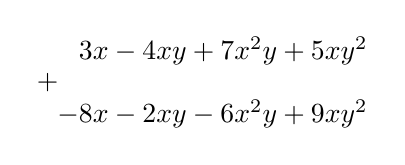
\begin{tikzpicture}
	\node[right] at (0,.4) {$\phantom{-}3x-4xy+7x^2y+5xy^2$};
	\node[right] at (0,-.4) {$-8x-2xy-6x^2y+9xy^2$};
	\node at (0,0) {$+$};
\end{tikzpicture}
%%a02
\begin{enum}
	\ii
	\ii
	\ii
	\ii
\end{enum}
%%r02
?
%%p03
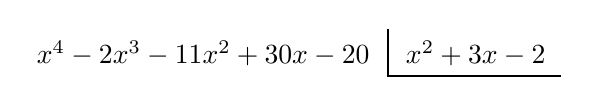
\begin{tikzpicture}[thick]
	\node[above left] at (-.1,0) {$x^4-2x^3-11x^2+30x-20$};
	\node[above right] at (.1,0) {$x^2+3x-2$};
	\draw (0,.6) -- (0,0) -- (2.2,0);
\end{tikzpicture}
%%a03
\begin{enum}
	\ii $x+5x^2$
	\ii $x^2-3x$
	\ii $2x-5x^2$
	\ii $x^2-5x$
\end{enum}
%%r03
$x^2-5x$
%%p04
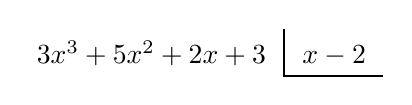
\begin{tikzpicture}[thick]
	\node[above left] at (-.1,0) {$3x^3+5x^2+2x+3$};
	\node[above right] at (.1,0) {$x-2$};
	\draw (0,.6) -- (0,0) -- (1.25,0);
\end{tikzpicture}
%%a04
\begin{enum}
	\ii $3x^2+24-11x$
	\ii $2x+13-24x^2$
	\ii $3x^2+11x-24$
	\ii $3x^2+11x+24$
\end{enum}
%%r04
$3x^2+11x+24$
%%p05
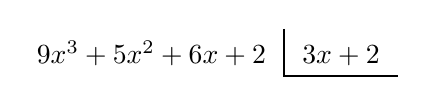
\begin{tikzpicture}[thick]
	\node[above left] at (-.1,0) {$9x^3+5x^2+6x+2$};
	\node[above right] at (.1,0) {$3x+2$};
	\draw (0,.6) -- (0,0) -- (1.45,0);
\end{tikzpicture}
%%a05
\begin{enum}
	\ii
	\ii
	\ii
	\ii
\end{enum}
%%r05
?
%%p06
$2x^4-x^3+x^2+7x-3$ entre $2x+3$
%%a06
\begin{enum}
	\ii $x^3-5x^2+4x-1$
	\ii $x^3-2x^2+3x-1$
	\ii $4x^3+2x^2+3x+1$
	\ii $4x^2-2x^4+5x+2$
\end{enum}
%%r06
$x^3-2x^2+3x-1$
%%p07
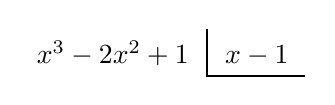
\begin{tikzpicture}[thick]
	\node[above left] at (-.1,0) {$x^3-2x^2+1$};
	\node[above right] at (.1,0) {$x-1$};
	\draw (0,.6) -- (0,0) -- (1.25,0);
\end{tikzpicture}
%%a07
\begin{enum}
	\ii $x^2-x$
	\ii $x+2x^2$
	\ii $2x^2+x$
	\ii $-x^2+x$
\end{enum}
%%r07
$-x^2+x$
%%p08
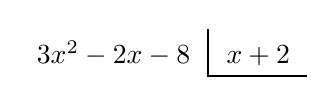
\begin{tikzpicture}[thick]
	\node[above left] at (-.1,0) {$3x^2-2x-8$};
	\node[above right] at (.1,.0) {$x+2$};
	\draw (0,.6) -- (0,0) -- (1.25,0);
\end{tikzpicture}
%%a08
\begin{enum}
	\ii $-3x+4$
	\ii $3x-6$
	\ii $3x+10$
	\ii $3x-8$
\end{enum}
%%r08
$3x-8$
%%p09
$\dfrac{6x^3-3x^2+9x-4}{3}$
%%a09
\begin{enum}
	\ii $2x^3-x^2+2x-1$
	\ii $2x^3+x^2+2x+1$
	\ii $2x^3+x^2-3x+1$
	\ii $2x^3+x^2+3x+1$
\end{enum}
%%r09
$2x^3-x^2+2x-1$
%%p10
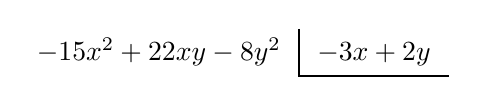
\begin{tikzpicture}[thick]
	\node[above left] at (-.1,0) {$-15x^2+22xy-8y^2$};
	\node[above right] at (.1,0) {$-3x+2y$};
	\draw (0,.6) -- (0,0) -- (1.9,0);
\end{tikzpicture}
%%a10
\begin{enum}
	\ii $5x-2y$
	\ii $3x+4y$
	\ii $5x-4y$
	\ii $7x-y$
\end{enum}
%%r10
$5x-4y$
%%p11
$6x^3-2x^2-15x+8$ entre $2x^2+x-5$
%%p12
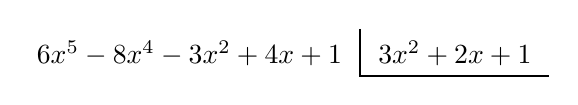
\begin{tikzpicture}[thick]
	\node[above left] at (-.1,0) {$6x^5-8x^4-3x^2+4x+1$};
	\node[above right] at (.1,0) {$3x^2+2x+1$};
	\draw (0,.6) -- (0,0) -- (2.4,0);
\end{tikzpicture}
%%p13
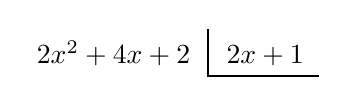
\begin{tikzpicture}[thick]
	\node[above left] at (-.1,0) {$2x^2+4x+2$};
	\node[above right] at (.1,0) {$2x+1$};
	\draw (0,.6) -- (0,0) -- (1.4,0);
\end{tikzpicture}
%%a13
\begin{enum}
	\ii $x+2$
	\ii $x+5$
	\ii $x+4$
	\ii $x+3$
\end{enum}
%%r13
$x+2$
%%p14
$\left(18x^3y^2z^5\right)\cdot\left(6x^3yz^2\right)$
%%a14
\begin{enum}
	\ii $120x^3y^5z$
	\ii $-180x^3yz^2$
	\ii $180x^6y^3z^7$
	\ii $-120x^3yz$
\end{enum}
%%r14
$180x^6y^3z^7$
%%p15
$\dfrac{6x^5-5x^3-35x-14x^2+23x^4+20}{3x^3-5+x^2}$
